% !TeX root = ../thuthesis-example.tex

\chapter{模型上下文协议}

模型上下文协议(Model Context Protocol, MCP)是一种标准化协议,用于规范AI应用与数据源和工具的连接与交互。MCP提供了通用的接口标准,使AI模型能够一致地访问外部资源,类似于USB-C为物理设备提供的标准连接方式。在MCP出现前,开发者需要为每个数据源或工具实现专用连接接口,这一过程既耗时又限制了应用功能的扩展。通过MCP,开发者可以更高效地为AI应用集成外部资源,从而提升应用的能力范围和实用价值\cite{mcpspec2023}。

bolt.se的MCP模块是该协议的实际应用实现,它支持用户配置和管理外部MCP服务器,使大语言模型(LLM)能够通过标准接口访问外部工具和数据。本章将分析MCP的理论基础、技术特点、在LLM驱动软件开发中的作用,以及bolt.se中MCP模块的具体实现方案。

\section{模型上下文协议的概念与意义}

\subsection{MCP在软件工程中的优势}
模型上下文协议为AI驱动的软件工程提供了以下核心优势:

\begin{enumerate}
  \item \textbf{标准化接口}:MCP提供统一的接口规范,简化了AI应用与外部工具的集成,降低了系统整合复杂度。
  
  \item \textbf{解耦与可扩展性}:通过接口抽象,实现AI模型与工具实现的完全解耦,使系统各部分能够独立演化,支持动态添加新工具。
  
  \item \textbf{传输协议灵活性}:支持多种传输协议(如stdio、HTTP SSE等),适应不同部署环境,提升系统适应能力。
  
  \item \textbf{工具发现机制}:内置的工具发现机制使AI模型能够动态识别可用工具的功能参数,实现智能化工具选择。
  
  \item \textbf{安全边界控制}:提供明确的权限边界设计,确保AI模型只能通过受控接口访问外部资源,有效控制系统安全风险。
\end{enumerate}

在bolt.se等现代开发平台中,MCP的这些特性支持开发者构建更灵活、更安全的AI应用生态系统。

\subsection{MCP对LLM驱动软件开发的重要性}
在大型语言模型(LLM)驱动的软件开发中,MCP具有以下关键作用:

\begin{enumerate}
  \item \textbf{突破知识截止限制}:通过MCP,LLM可以访问实时外部数据,克服训练数据时间限制,保持信息时效性。
  
  \item \textbf{扩展功能边界}:使LLM能够调用专业工具和API,执行其内部能力无法完成的任务,如数据分析、文件处理等,扩展应用场景。
  
  \item \textbf{降低输出幻觉}:引导LLM从可靠外部来源获取信息,减少对参数化知识的依赖,显著提高输出准确性。
  
  \item \textbf{支持交互式解决方案}:提供LLM与外部工具多轮交互的能力,实现复杂问题的分步骤解决及中间结果验证。
  
  \item \textbf{保障数据安全访问}:提供安全机制,在保护隐私前提下实现LLM对用户私有数据的访问,平衡功能与安全需求。
\end{enumerate}

bolt.se已将MCP深度整合到系统设计中,通过标准化工具接口,实现LLM与外部工具及数据源的协作,使开发者能通过自然语言交互获得工具增强的智能辅助,既保留LLM的灵活创造性,又提供专业工具的精确性和功能扩展。

\section{MCP协议规范与工具类型}

MCP是一种开放协议规范,为AI模型与外部上下文的交互提供标准化接口,定义了通信格式、传输方式及工具调用机制\cite{mcpspec2023}。

\subsection{MCP协议核心组件}

MCP协议由以下关键组件构成:

\begin{enumerate}
  \item \textbf{传输层}:定义客户端与服务器间的通信机制,支持两种主要模式:
    \begin{itemize}
      \item \textit{stdio传输}:通过标准输入/输出流与本地进程通信,适用于本地工具执行。
      \item \textit{HTTP SSE传输}:通过HTTP Server-Sent Events建立远程连接,适用于云服务和网络API。
    \end{itemize}
  
  \item \textbf{消息格式}:基于JSON的消息交换协议,包括:
    \begin{itemize}
      \item 握手消息:建立连接并交换版本信息
      \item 工具发现消息:获取可用工具及其描述
      \item 工具调用消息:请求执行特定工具与参数
      \item 工具响应消息:返回执行结果
      \item 错误消息:传递执行异常信息
    \end{itemize}
  
  \item \textbf{工具模式}:采用JSON Schema定义工具接口,包含:
    \begin{itemize}
      \item 工具名称与描述:明确功能与用途
      \item 参数规范:指定必需和可选参数,含类型与约束
      \item 返回值定义:规定输出结构与类型
    \end{itemize}
\end{enumerate}

以下是bolt.se支持的MCP服务器配置示例:

\begin{verbatim}
{
  "mcpServers": {
    "localFileSystem": {
      "type": "stdio",
      "command": "node",
      "args": ["./mcp-file-server.js"]
    },
    "weatherService": {
      "type": "sse",
      "url": "https://weather-mcp.example.com/connect"
    }
  }
}
\end{verbatim}

bolt.se的MCP模块解析此类配置,创建相应MCP客户端,连接指定服务器并获取可用工具集。

\subsection{MCP支持的工具类型}

MCP协议支持多种功能类型的工具,满足不同AI应用需求:

\begin{enumerate}
  \item \textbf{信息检索工具}:实现对外部数据的访问,如网络搜索、文档查询、数据库访问等。
  
  \item \textbf{计算工具}:提供数学运算、统计分析、数据处理等能力,弥补LLM在精确计算方面的局限。
  
  \item \textbf{文件操作工具}:支持文件读写、创建和删除,用于代码生成和文档处理。
  
  \item \textbf{API调用工具}:封装第三方API访问,如天气服务、地图服务、社交媒体API等。
  
  \item \textbf{系统交互工具}:提供与操作系统交互功能,如命令执行、进程管理等。
  
  \item \textbf{领域专用工具}:集成特定专业领域工具,如代码分析、图形处理、自然语言处理等。
\end{enumerate}

MCP的开放性和可扩展性允许开发者根据需求创建自定义工具,并通过标准接口与LLM集成。bolt.se基于此理念,提供灵活的MCP配置和管理机制,支持用户按需扩展系统能力。

\section{bolt.se中的MCP实现}

bolt.se将MCP深度融入其架构设计,通过结构化的模块实现,使用户能够配置、管理外部MCP服务器,并让大语言模型访问这些服务提供的工具。本节将分析bolt.se中MCP的具体实现方案。

\begin{figure}[htbp]
  \centering
  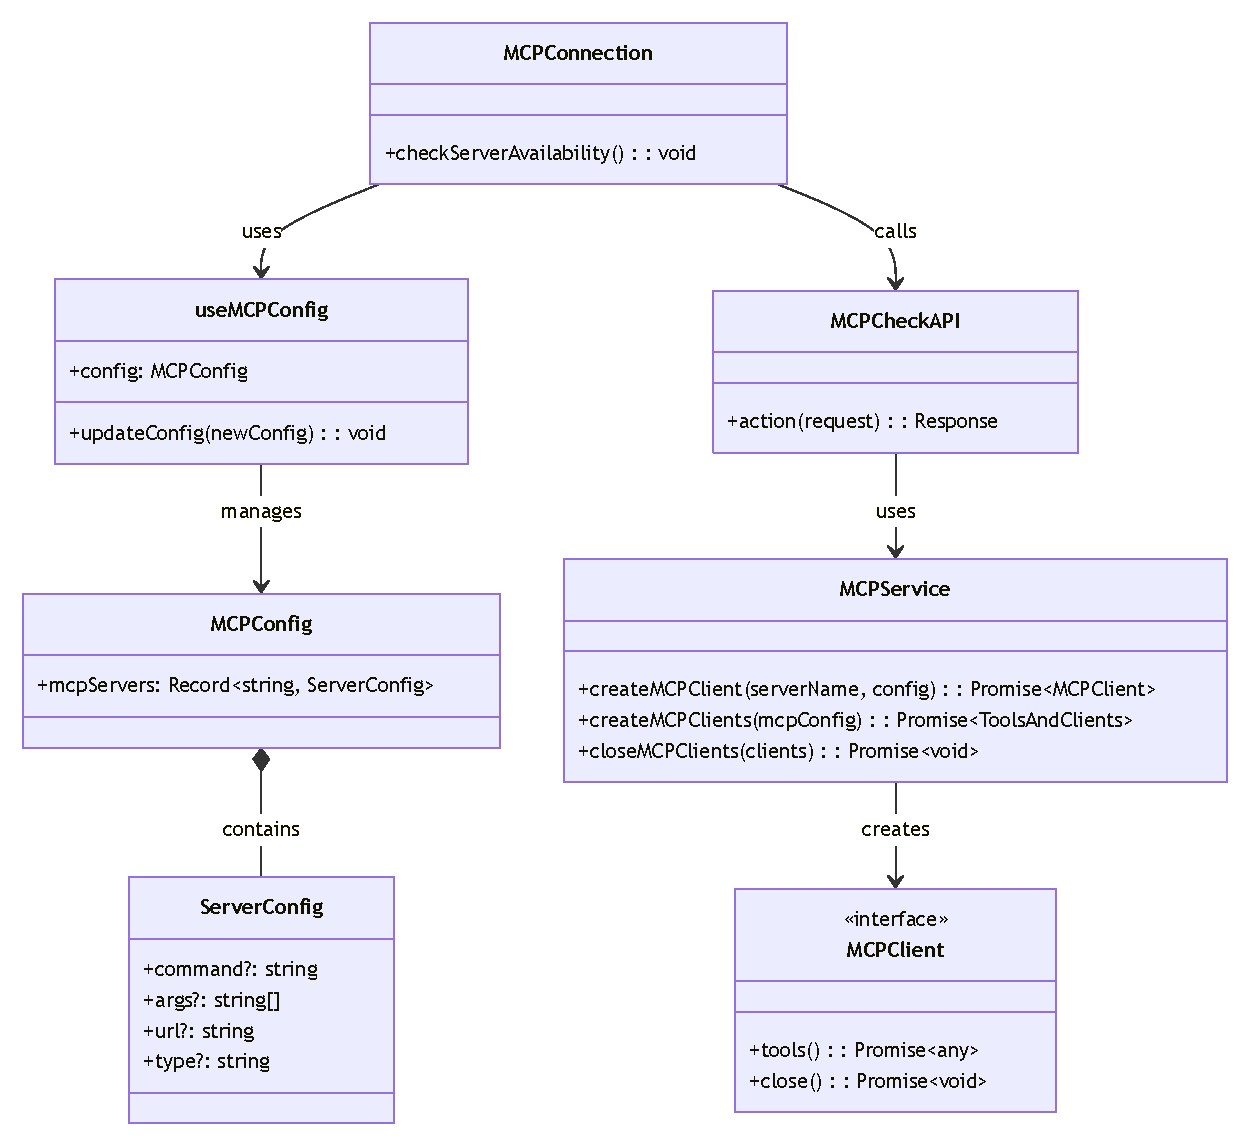
\includegraphics[width=\textwidth]{figures/mcp_class.pdf}
  \caption{MCP类图:展示系统中MCP相关模块的类结构及其关系,包括配置管理、服务创建和连接检查}
  \label{fig:mcp_class}
\end{figure}

% classDiagram
%     class MCPConfig {
%         +mcpServers: Record~string, ServerConfig~
%     }

%     class ServerConfig {
%         +command?: string
%         +args?: string[]
%         +url?: string
%         +type?: string
%     }

%     class MCPClient {
%         <<interface>>
%         +tools(): Promise~any~
%         +close(): Promise~void~
%     }

%     class MCPService {
%         +createMCPClient(serverName, config): Promise~MCPClient~
%         +createMCPClients(mcpConfig): Promise~ToolsAndClients~
%         +closeMCPClients(clients): Promise~void~
%     }

%     class useMCPConfig {
%         +config: MCPConfig
%         +updateConfig(newConfig): void
%     }

%     class MCPConnection {
%         +checkServerAvailability(): void
%     }

%     class MCPCheckAPI {
%         +action(request): Response
%     }

%     MCPConfig *-- ServerConfig : contains
%     MCPService --> MCPClient : creates
%     useMCPConfig --> MCPConfig : manages
%     MCPConnection --> useMCPConfig : uses
%     MCPConnection --> MCPCheckAPI : calls
%     MCPCheckAPI --> MCPService : uses 

\subsection{架构设计与模块划分}

bolt.se的MCP系统采用模块化设计,主要包含以下组件:

\begin{enumerate}
  \item \textbf{配置管理组件}:
    \begin{itemize}
      \item \texttt{MCPConfig}:MCP服务器配置的数据模型
      \item \texttt{useMCPConfig}:提供配置管理的React Hook
      \item \texttt{IndexedDB存储}:持久化存储配置信息
    \end{itemize}
  
  \item \textbf{服务层组件}:
    \begin{itemize}
      \item \texttt{MCPService}:负责创建和管理MCP客户端
      \item \texttt{MCPClient}:定义与MCP服务器交互的接口
      \item \texttt{createMCPClient}:根据配置创建不同类型客户端的工厂函数
    \end{itemize}
  
  \item \textbf{用户界面组件}:
    \begin{itemize}
      \item \texttt{MCPConnection}:提供服务器配置和管理的界面
    \end{itemize}
  
  \item \textbf{API组件}:
    \begin{itemize}
      \item \texttt{MCPCheckAPI}:提供服务器可用性检查的API端点
    \end{itemize}
  
  \item \textbf{AI交互层}:负责将MCP工具集成到AI对话流程中
\end{enumerate}

如图\ref{fig:mcp_class}所示,MCP架构体现了清晰的职责分离原则,各组件专注于特定功能,共同构成完整的MCP支持系统。

\begin{figure}[htbp]
  \centering
  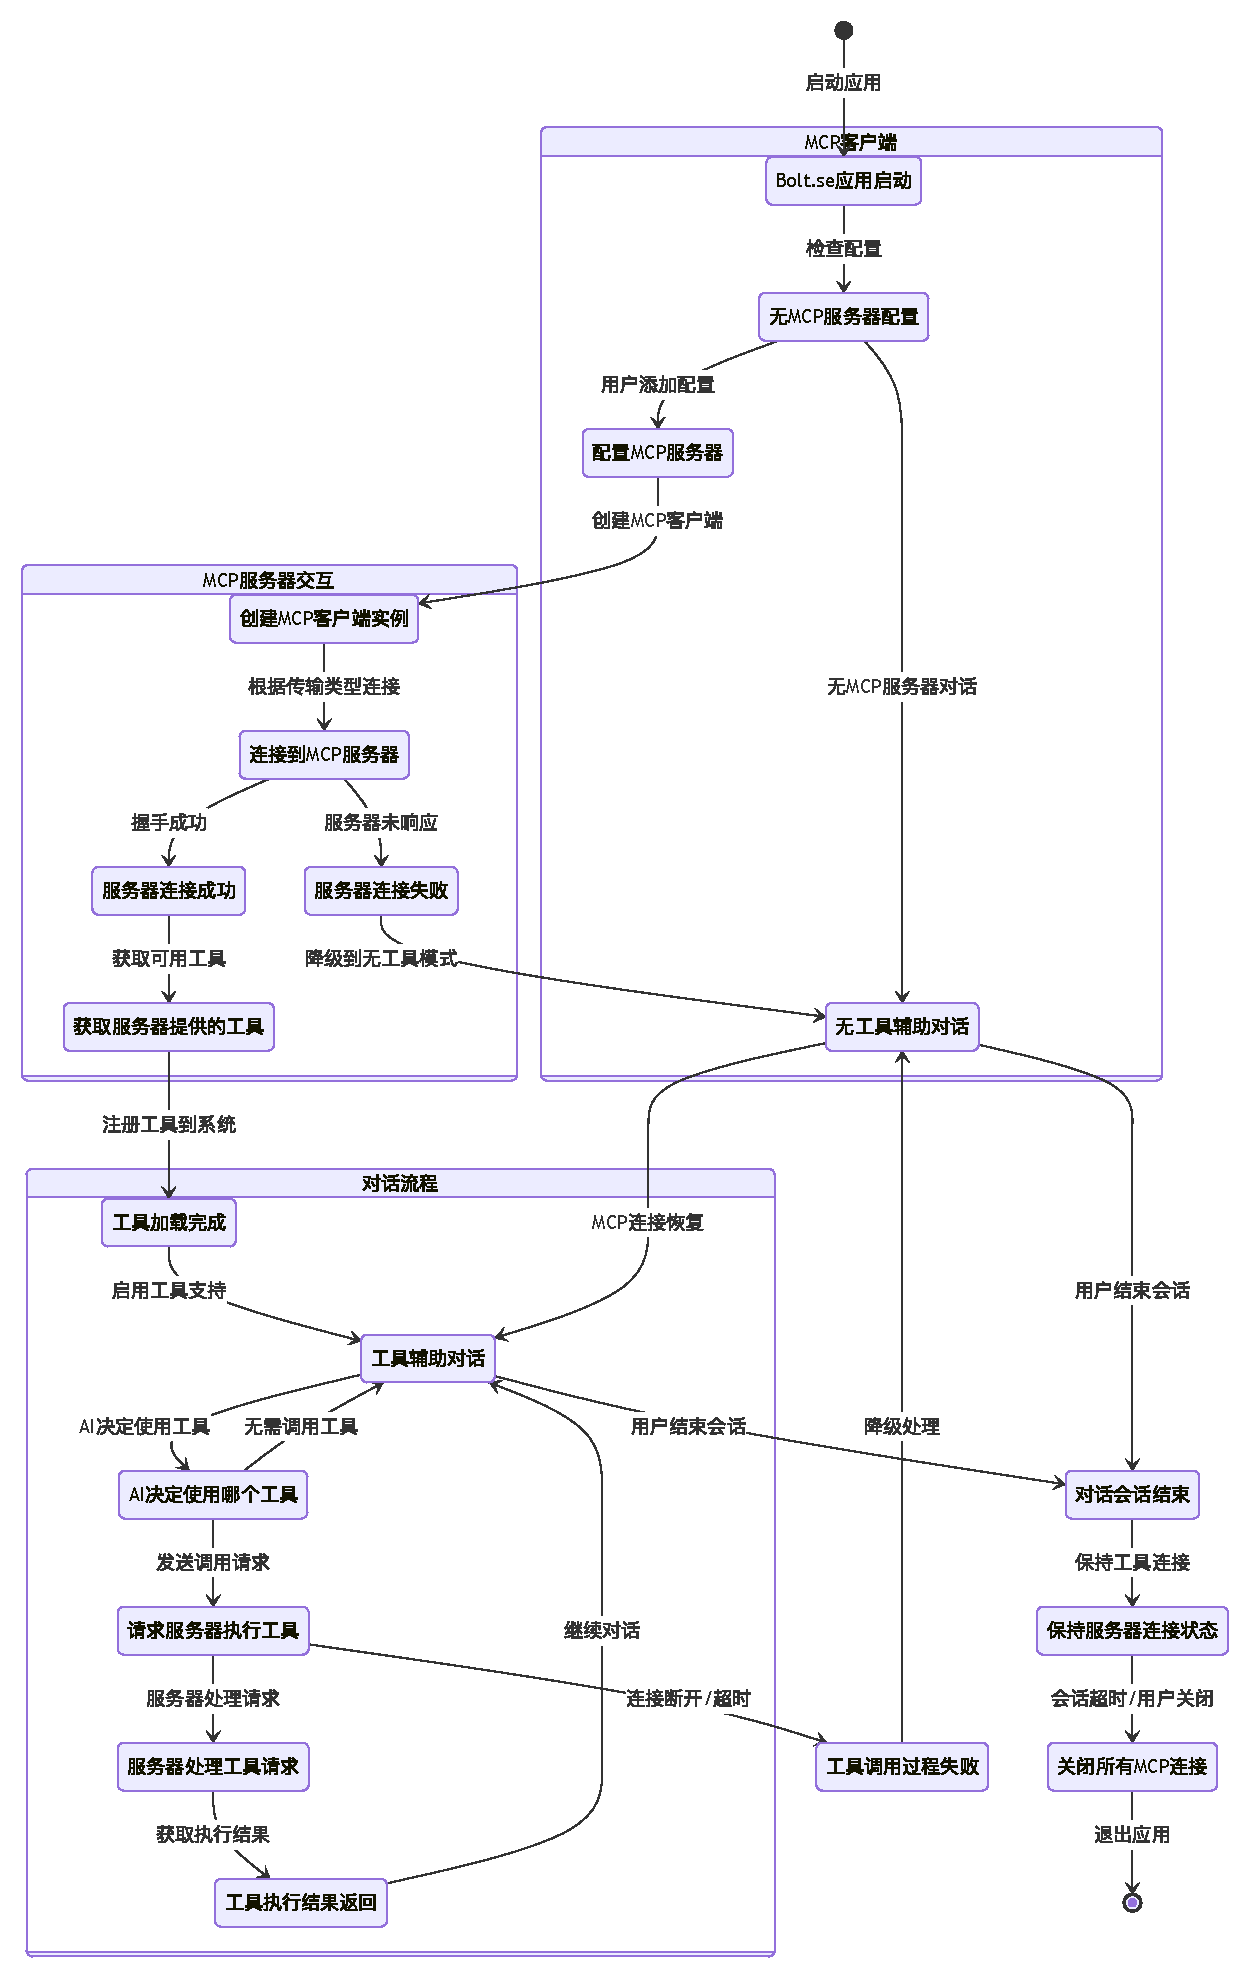
\includegraphics[width=\textwidth]{figures/mcp_state.pdf}
  \caption{MCP状态图:描述MCP连接的各状态及转换关系,从初始配置到工具调用的完整流程}
  \label{fig:mcp_state}
\end{figure}

% stateDiagram-v2
%     [*] --> Host初始状态 : 启动应用
    
%     state MCP客户端 {
%         Host初始状态 --> 未配置 : 检查配置
%         未配置 --> 配置中 : 用户添加配置
%         未配置 --> 基础对话模式 : 无MCP服务器对话
%         配置中 --> 连接初始化 : 创建MCP客户端
%     }
    
%     state MCP服务器交互 {
%         连接初始化 --> 服务器连接中 : 根据传输类型连接
%         服务器连接中 --> 连接失败 : 服务器未响应
%         服务器连接中 --> 连接成功 : 握手成功
%         连接成功 --> 工具发现 : 获取可用工具
%         工具发现 --> 工具就绪 : 注册工具到系统
%     }
    
%     state 对话流程 {
%         工具就绪 --> 增强对话模式 : 启用工具支持
%         增强对话模式 --> 工具选择 : AI决定使用工具
%         工具选择 --> 工具调用 : 发送调用请求
%         工具调用 --> 工具执行 : 服务器处理请求
%         工具执行 --> 结果返回 : 获取执行结果
%         结果返回 --> 增强对话模式 : 继续对话
%         工具选择 --> 增强对话模式 : 无需调用工具
%     }
    
%     连接失败 --> 基础对话模式 : 降级到无工具模式
%     基础对话模式 --> 增强对话模式 : MCP连接恢复
    
%     增强对话模式 --> 会话结束 : 用户结束会话
%     基础对话模式 --> 会话结束 : 用户结束会话
    
%     工具调用 --> 调用失败 : 连接断开/超时
%     调用失败 --> 基础对话模式 : 降级处理
    
%     会话结束 --> 连接保持 : 保持工具连接
%     连接保持 --> 连接关闭 : 会话超时/用户关闭
%     连接关闭 --> [*] : 退出应用
    
%     Host初始状态 : Bolt.se应用启动
%     未配置 : 无MCP服务器配置
%     配置中 : 配置MCP服务器
%     连接初始化 : 创建MCP客户端实例
%     服务器连接中 : 连接到MCP服务器
%     连接失败 : 服务器连接失败
%     连接成功 : 服务器连接成功
%     工具发现 : 获取服务器提供的工具
%     工具就绪 : 工具加载完成
%     基础对话模式 : 无工具辅助对话
%     增强对话模式 : 工具辅助对话
%     工具选择 : AI决定使用哪个工具
%     工具调用 : 请求服务器执行工具
%     工具执行 : 服务器处理工具请求
%     结果返回 : 工具执行结果返回
%     调用失败 : 工具调用过程失败
%     会话结束 : 对话会话结束
%     连接保持 : 保持服务器连接状态
%     连接关闭 : 关闭所有MCP连接 
如图\ref{fig:mcp_state}所示,MCP连接的生命周期分为四个主要阶段:客户端初始化、服务器交互、对话流程和会话结束。系统首先检查MCP配置,创建客户端并连接服务器。连接成功后进入工具发现阶段,将获取的工具注册到系统中。工具就绪后,用户对话转入增强模式,LLM能够根据需要选择和调用工具。状态图还包含错误处理机制:连接失败或工具调用出错时,系统会降级到基础对话模式,保证用户体验不中断。这种设计确保了MCP功能的健壮性和可靠性,能够优雅处理各种正常和异常情况。

bolt.se的MCP数据模型包括:

\begin{enumerate}
  \item \textbf{MCPConfig}:顶层配置对象,包含服务器映射表
  
  \item \textbf{ServerConfig}:服务器配置对象,根据传输类型包含不同属性:
    \begin{itemize}
      \item stdio配置:包括命令(command)、参数(args)、环境变量(env)和工作目录(cwd)
      \item SSE配置:包括URL(url)和类型(type)
    \end{itemize}
  
  \item \textbf{MCPClient}:客户端接口,定义获取工具(tools)和关闭连接(close)方法
\end{enumerate}

\subsection{服务器配置与连接管理}
bolt.se实现了完整的MCP服务器配置和连接管理功能:

\begin{enumerate}
  \item \textbf{配置存储}:使用IndexedDB持久化存储MCP配置,确保配置在会话间保持一致:
    \begin{itemize}
      \item \texttt{saveMCPConfig}:保存配置
      \item \texttt{getMCPConfig}:获取配置
      \item \texttt{deleteMCPConfig}:删除配置
    \end{itemize}
  
  \item \textbf{配置管理Hook}:\texttt{useMCPConfig} React Hook封装配置管理逻辑,包括初始化、更新和事件通知功能
  
  \item \textbf{服务器连接检查}:实现服务器可用性检查,验证配置有效性并获取可用工具列表
  
  \item \textbf{配置界面}:提供用户界面用于编辑MCP配置,包括JSON编辑器、服务器状态指示器和工具浏览器
\end{enumerate}

\subsection{MCP客户端实现与工具集成}
bolt.se的MCP客户端实现采用以下关键机制:

\begin{enumerate}
  \item \textbf{客户端工厂}:\texttt{createMCPClient}函数根据服务器配置创建适当类型的客户端:
    \begin{itemize}
      \item stdio类型:创建基于子进程的客户端
      \item SSE类型:创建基于HTTP连接的客户端
    \end{itemize}
  
  \item \textbf{客户端管理}:\texttt{createMCPClients}函数并行管理多个客户端,合并工具集,并确保部分服务器失败不影响整体功能
  
  \item \textbf{工具发现}:通过客户端的\texttt{tools}方法获取服务器提供的工具,解析工具模式并创建JavaScript表示
  
  \item \textbf{LLM集成}:将MCP工具整合到LLM对话上下文中,处理调用请求,执行操作并返回结果
  
  \item \textbf{资源清理}:\texttt{closeMCPClients}函数在对话结束或页面卸载时正确关闭所有客户端连接
\end{enumerate}

\begin{figure}[htbp]
  \centering
  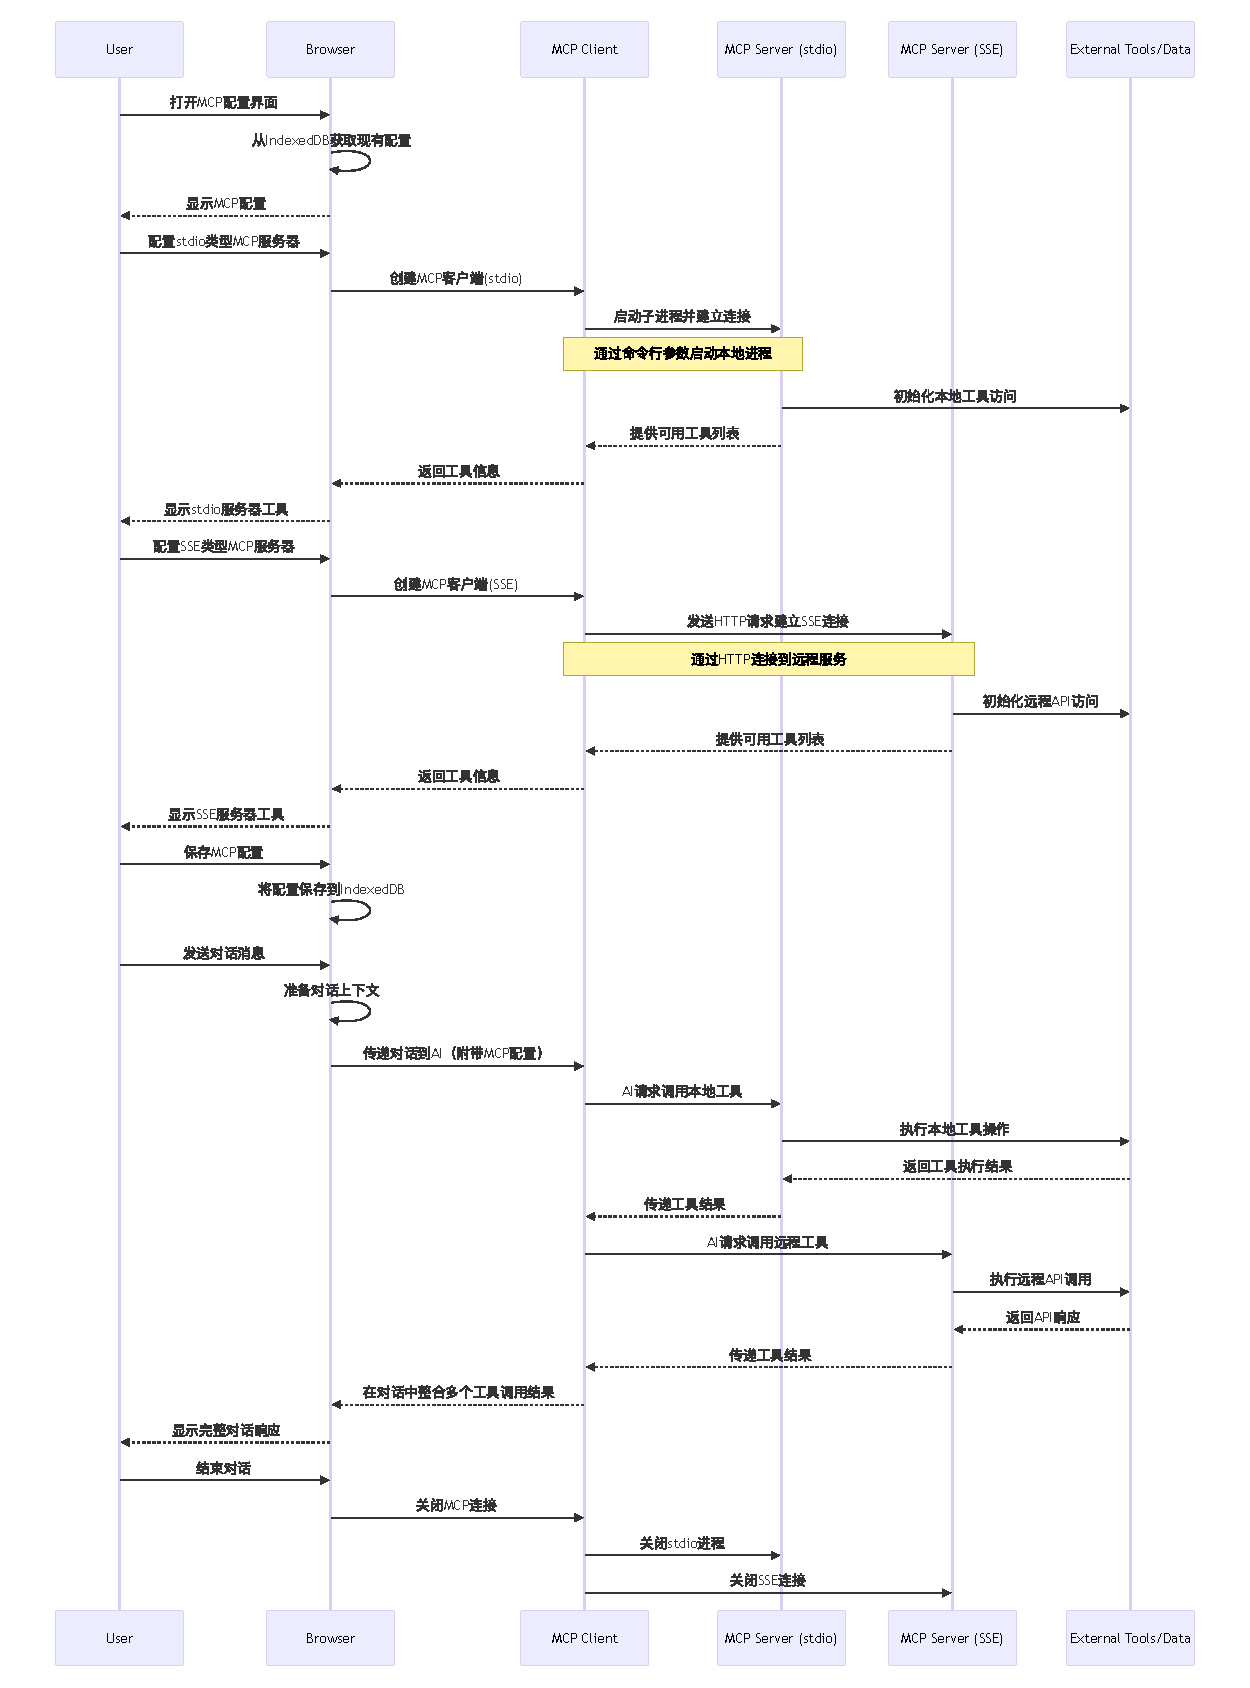
\includegraphics[width=\textwidth]{figures/mcp_sequence.pdf}
  \caption{MCP序列图:展示用户、客户端和服务器间的交互序列,包括配置、连接和工具调用过程}
  \label{fig:mcp_sequence}
\end{figure}

% sequenceDiagram
%     participant User
%     participant Host as Browser
%     participant Client as MCP Client
%     participant ServerStdio as MCP Server (stdio)
%     participant ServerSSE as MCP Server (SSE)
%     participant Tools as External Tools/Data

%     %% 配置过程
%     User->>Host: 打开MCP配置界面
%     Host->>Host: 从IndexedDB获取现有配置
%     Host-->>User: 显示MCP配置
    
%     %% stdio方式配置
%     User->>Host: 配置stdio类型MCP服务器
%     Host->>Client: 创建MCP客户端(stdio)
%     Client->>ServerStdio: 启动子进程并建立连接
%     Note over Client,ServerStdio: 通过命令行参数启动本地进程
%     ServerStdio->>Tools: 初始化本地工具访问
%     ServerStdio-->>Client: 提供可用工具列表
%     Client-->>Host: 返回工具信息
%     Host-->>User: 显示stdio服务器工具
    
%     %% SSE方式配置
%     User->>Host: 配置SSE类型MCP服务器
%     Host->>Client: 创建MCP客户端(SSE)
%     Client->>ServerSSE: 发送HTTP请求建立SSE连接
%     Note over Client,ServerSSE: 通过HTTP连接到远程服务
%     ServerSSE->>Tools: 初始化远程API访问
%     ServerSSE-->>Client: 提供可用工具列表
%     Client-->>Host: 返回工具信息
%     Host-->>User: 显示SSE服务器工具
    
%     %% 保存配置
%     User->>Host: 保存MCP配置
%     Host->>Host: 将配置保存到IndexedDB
    
%     %% 对话过程
%     User->>Host: 发送对话消息
%     Host->>Host: 准备对话上下文
    
%     %% 根据配置选择传输方式
%     Host->>Client: 传递对话到AI(附带MCP配置)
    
%     %% 通过stdio调用工具
%     Client->>ServerStdio: AI请求调用本地工具
%     ServerStdio->>Tools: 执行本地工具操作
%     Tools-->>ServerStdio: 返回工具执行结果
%     ServerStdio-->>Client: 传递工具结果
    
%     %% 通过SSE调用工具
%     Client->>ServerSSE: AI请求调用远程工具
%     ServerSSE->>Tools: 执行远程API调用
%     Tools-->>ServerSSE: 返回API响应
%     ServerSSE-->>Client: 传递工具结果
    
%     %% 结果整合
%     Client-->>Host: 在对话中整合多个工具调用结果
%     Host-->>User: 显示完整对话响应

%     %% 会话结束
%     User->>Host: 结束对话
%     Host->>Client: 关闭MCP连接
%     Client->>ServerStdio: 关闭stdio进程
%     Client->>ServerSSE: 关闭SSE连接 
图\ref{fig:mcp_sequence}展示了用户、浏览器和不同类型MCP服务器间的完整交互流程。配置阶段包括用户配置stdio和SSE服务器,系统通过相应方式建立连接并获取工具列表。对话阶段中,系统根据配置将请求路由至对应服务器执行工具操作,然后获取结果。会话结束时系统关闭所有连接释放资源。序列图清晰展示了不同传输模式下MCP的生命周期及组件协作关系。

\section{MCP在bolt.se中的应用场景}

bolt.se的MCP实现支持多种应用场景,从本地工具集成到云服务接入。本节通过具体实例,分析MCP如何增强开发平台功能。

\subsection{本地文件系统访问}

通过stdio类型MCP服务器,实现安全的本地文件系统操作:

\begin{verbatim}
{
  "mcpServers": {
    "localFiles": {
      "type": "stdio",
      "command": "node",
      "args": ["./mcp-file-server.js"]
    }
  }
}
\end{verbatim}

此配置使LLM能够:
\begin{itemize}
  \item 读取文件内容,理解项目结构
  \item 创建和修改文件,支持代码生成和重构
  \item 执行文件系统搜索和导航
\end{itemize}

用户可通过自然语言指令如"分析项目结构"或"创建新组件"让LLM操作本地文件。

\subsection{外部API集成}

使用SSE类型MCP服务器集成外部服务和API:

\begin{verbatim}
{
  "mcpServers": {
    "weatherAPI": {
      "type": "sse",
      "url": "https://weather-mcp.example.com/connect"
    },
    "databaseAccess": {
      "type": "sse",
      "url": "https://db-mcp.example.com/connect"
    }
  }
}
\end{verbatim}

此配置使LLM能够:
\begin{itemize}
  \item 获取实时数据,如天气信息或市场数据
  \item 查询和更新在线数据库
  \item 调用专业服务API,如翻译或图像处理
\end{itemize}

\subsection{开发工具集成}

通过专用MCP服务器集成开发工具链:

\begin{verbatim}
{
  "mcpServers": {
    "gitOperations": {
      "type": "stdio",
      "command": "node",
      "args": ["./mcp-git-server.js"]
    },
    "codeAnalysis": {
      "type": "sse",
      "url": "https://code-analysis-mcp.example.com/connect"
    }
  }
}
\end{verbatim}

此配置支持LLM:
\begin{itemize}
  \item 执行Git操作,如分支管理和提交
  \item 运行代码分析,检测问题和优化机会
  \item 执行构建和测试流程
\end{itemize}

\section{MCP与传统AI开发方式对比}

MCP方式相比传统AI开发方式具有以下优势:

\begin{enumerate}
  \item \textbf{功能扩展}:传统模型受限于训练数据和内部功能,MCP通过工具集成显著扩展了AI应用的功能边界。

  \item \textbf{数据时效性}:传统模型依赖训练时知识,MCP提供实时数据访问通道,保证信息准确性和时效性。

  \item \textbf{开发效率}:传统方式需针对新需求更新模型,MCP允许通过添加工具动态扩展能力,降低开发成本。

  \item \textbf{资源优化}:MCP通过工具分担任务,减少对大型模型的依赖,优化计算资源利用。

  \item \textbf{安全边界}:MCP提供明确的功能边界和权限控制,增强应用安全性和可靠性。
\end{enumerate}

在bolt.se中,MCP成为连接AI与外部环境的桥梁,将LLM的生成能力与专业工具的精确性结合,创造超越传统AI应用的开发体验。

\section{实例应用场景}
\label{sec:mcp-iotdb-demo}

本节以"MCP协同IoTDB与OpenAPI构建交互式前端应用"为例,展示:
\begin{enumerate}
  \item 时序数据库Apache IoTDB作为双通道外部能力的暴露方式:MCP工具与REST API
  \item bolt.se在单一自然语言提示中同时发现并调用两类能力的机制
  \item LLM基于实时查询结果生成可视化应用及数据刷新功能的实现
\end{enumerate}

\subsection{系统配置}

开发环境部署IoTDB 2.0.2实例,并将名为\texttt{battery\_data}的样例数据表写入30条监测数据(包含电压、电流等参数)。系统通过两种方式暴露数据库能力:

\begin{enumerate}
  \item \textbf{MCP通道}:使用\texttt{remote-sse}服务器提供三个核心工具:
        \textit{list\_tables}、\textit{describe\_table}与
        \textit{read\_query},供LLM进行表结构分析和数据查询。
  \item \textbf{REST通道}:通过IoTDB内置的REST Service V2,将
        查询接口\texttt{/rest/table/v1/query}按OpenAPI 3.0规范描述。
\end{enumerate}

\subsection{MCP服务器配置与工具发现}

图~\ref{fig:mcp-config}展示了bolt.se的MCP配置界面。系统通过以下配置成功发现三个IoTDB工具:

\begin{verbatim}
{
  "mcpServers": {
    "remote-sse": {
      "type": "sse",
      "url": "http://localhost:8000/sse"
    }
  }
}
\end{verbatim}

\begin{figure}[htbp]
  \centering
  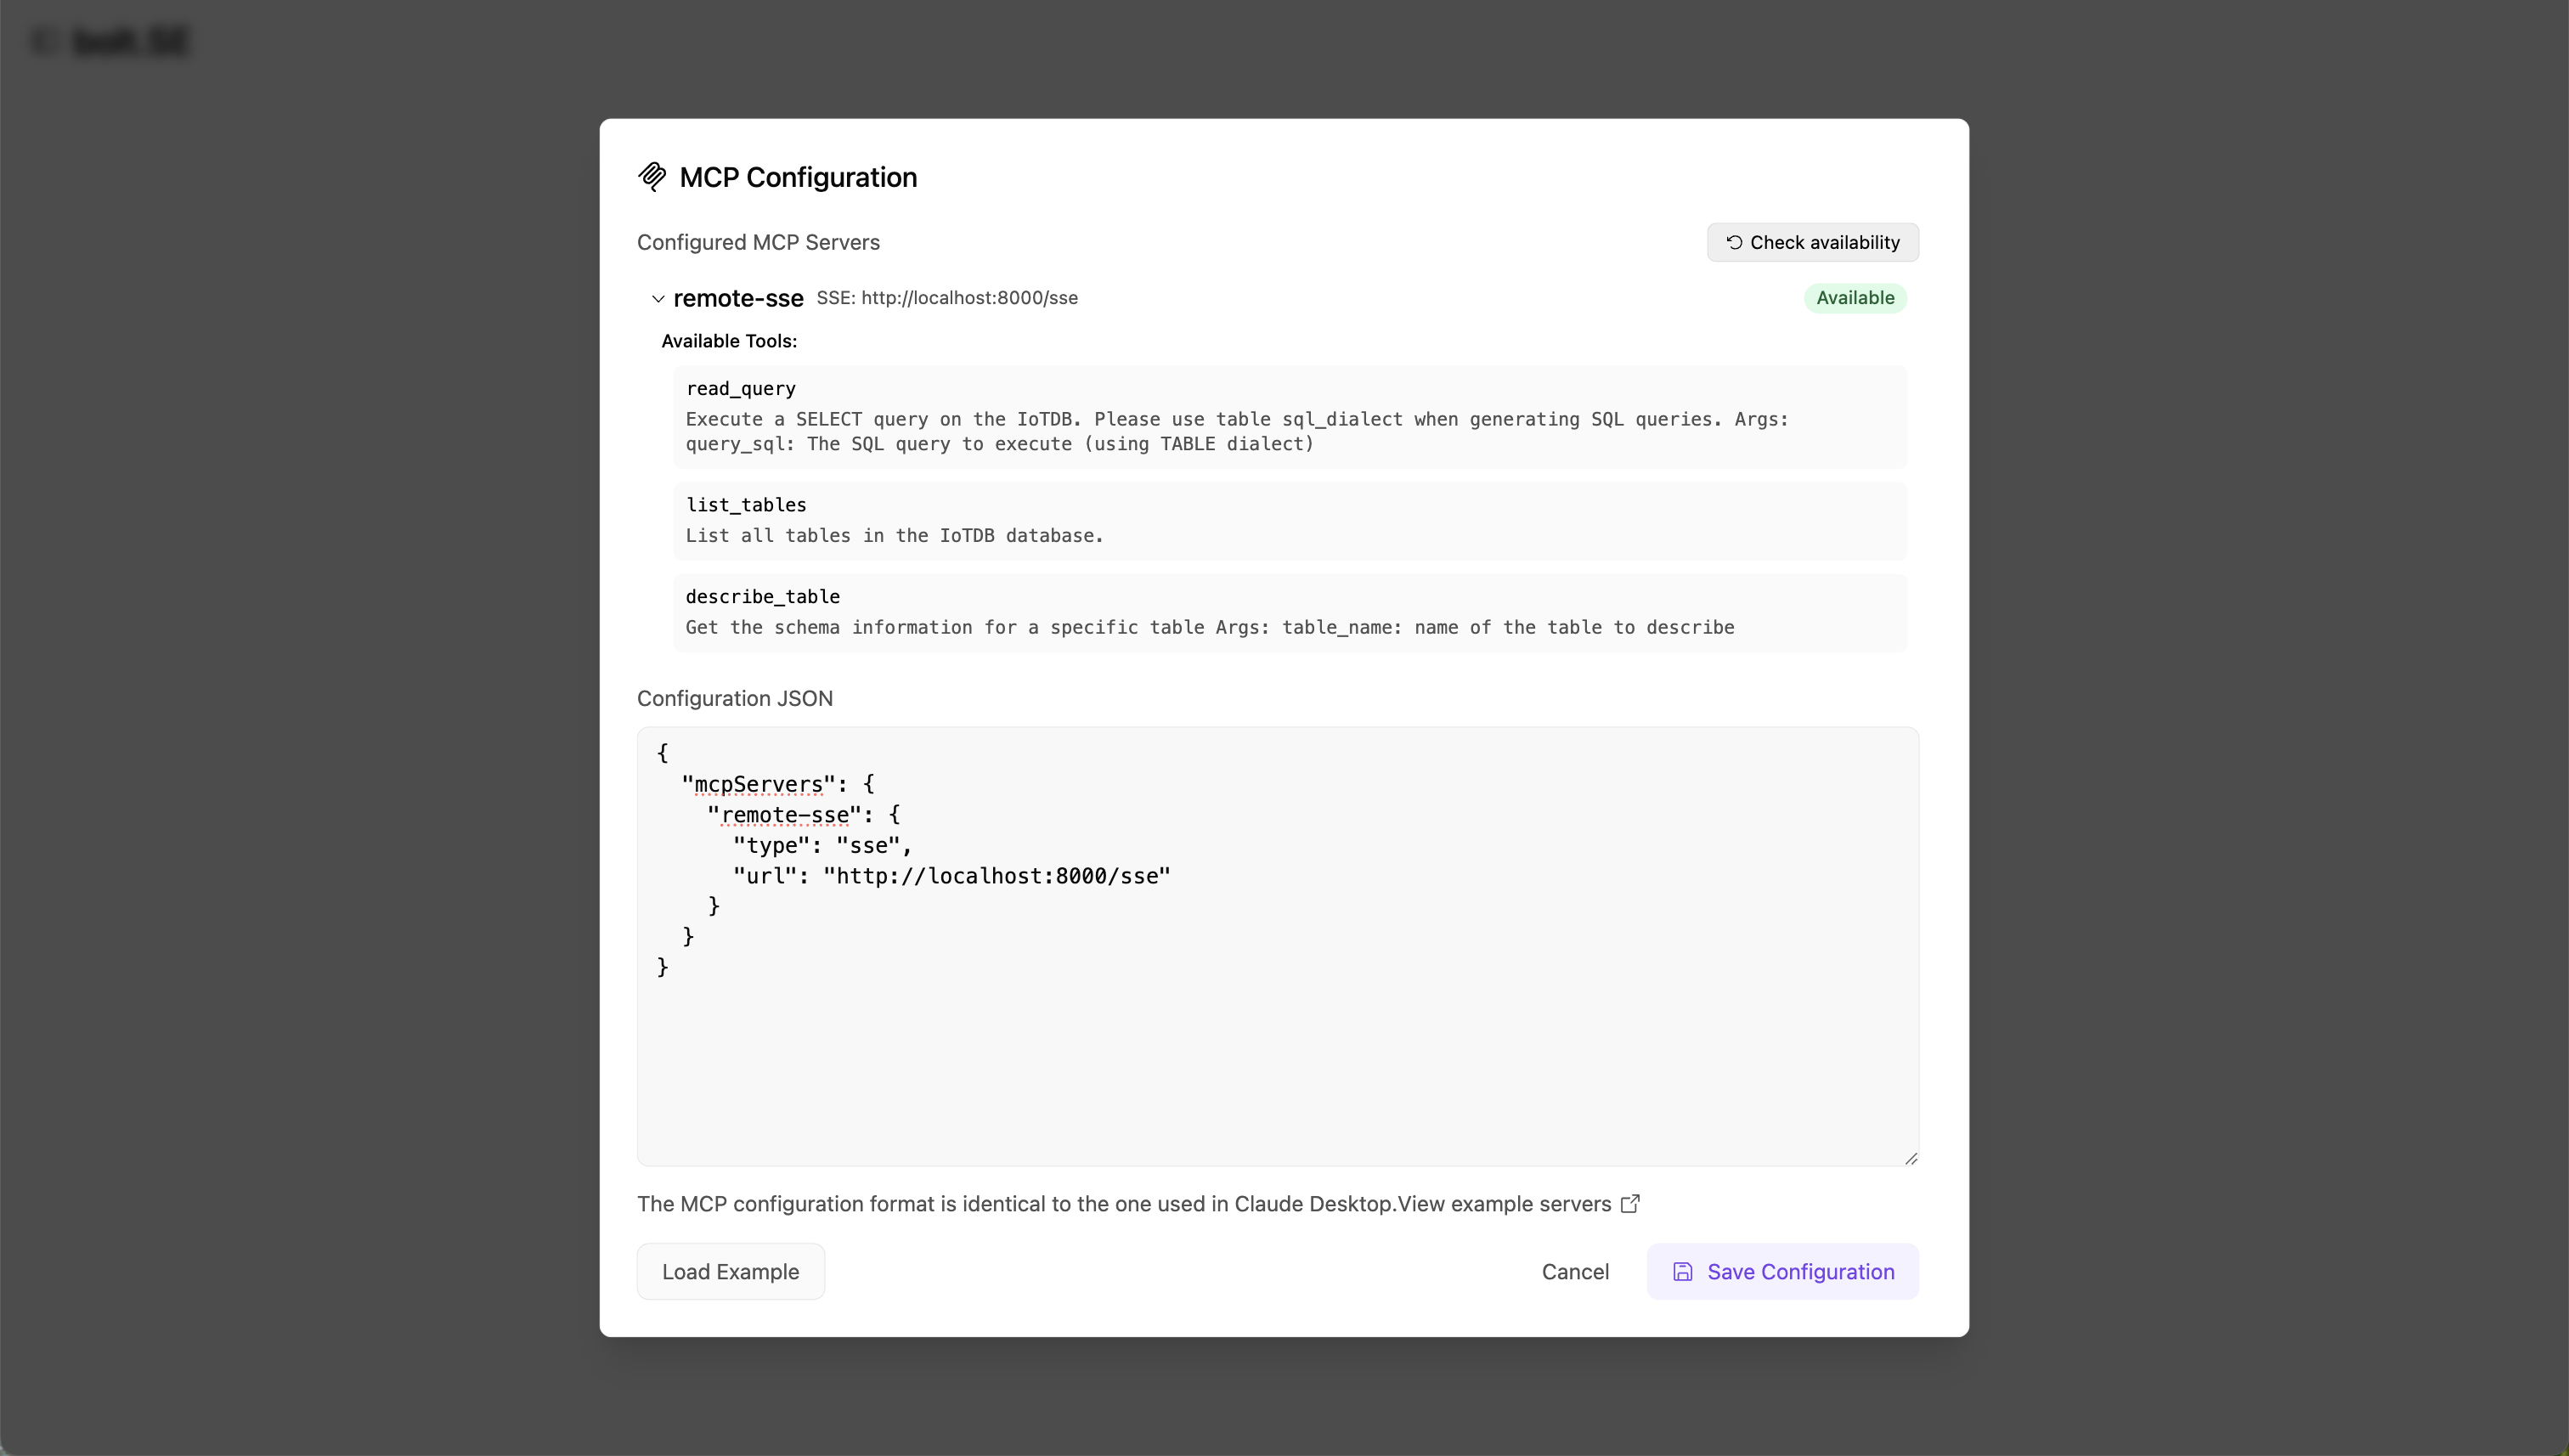
\includegraphics[width=0.75\textwidth]{figures/screenshots/iotdb-demo/mcp-config.png}
  \caption{\texttt{remote-sse}服务器配置与IoTDB工具发现}
  \label{fig:mcp-config}
\end{figure}

\subsection{REST API规范定义}

开发者将IoTDB查询接口按OpenAPI 3.0规范描述(如下所示),并在bolt.se的\textit{Edit actions}界面完成配置,仅保留\textit{queryTableData}动作供LLM调用。

\begin{verbatim}
paths:
  /rest/table/v1/query:
    post:
      operationId: queryTableData
      summary: Execute a SQL query on the IoTDB table
      requestBody:
        required: true
        content:
          application/json:
            schema:
              type: object
              required: [database, sql]
\end{verbatim}

\begin{figure}[htbp]
  \centering
  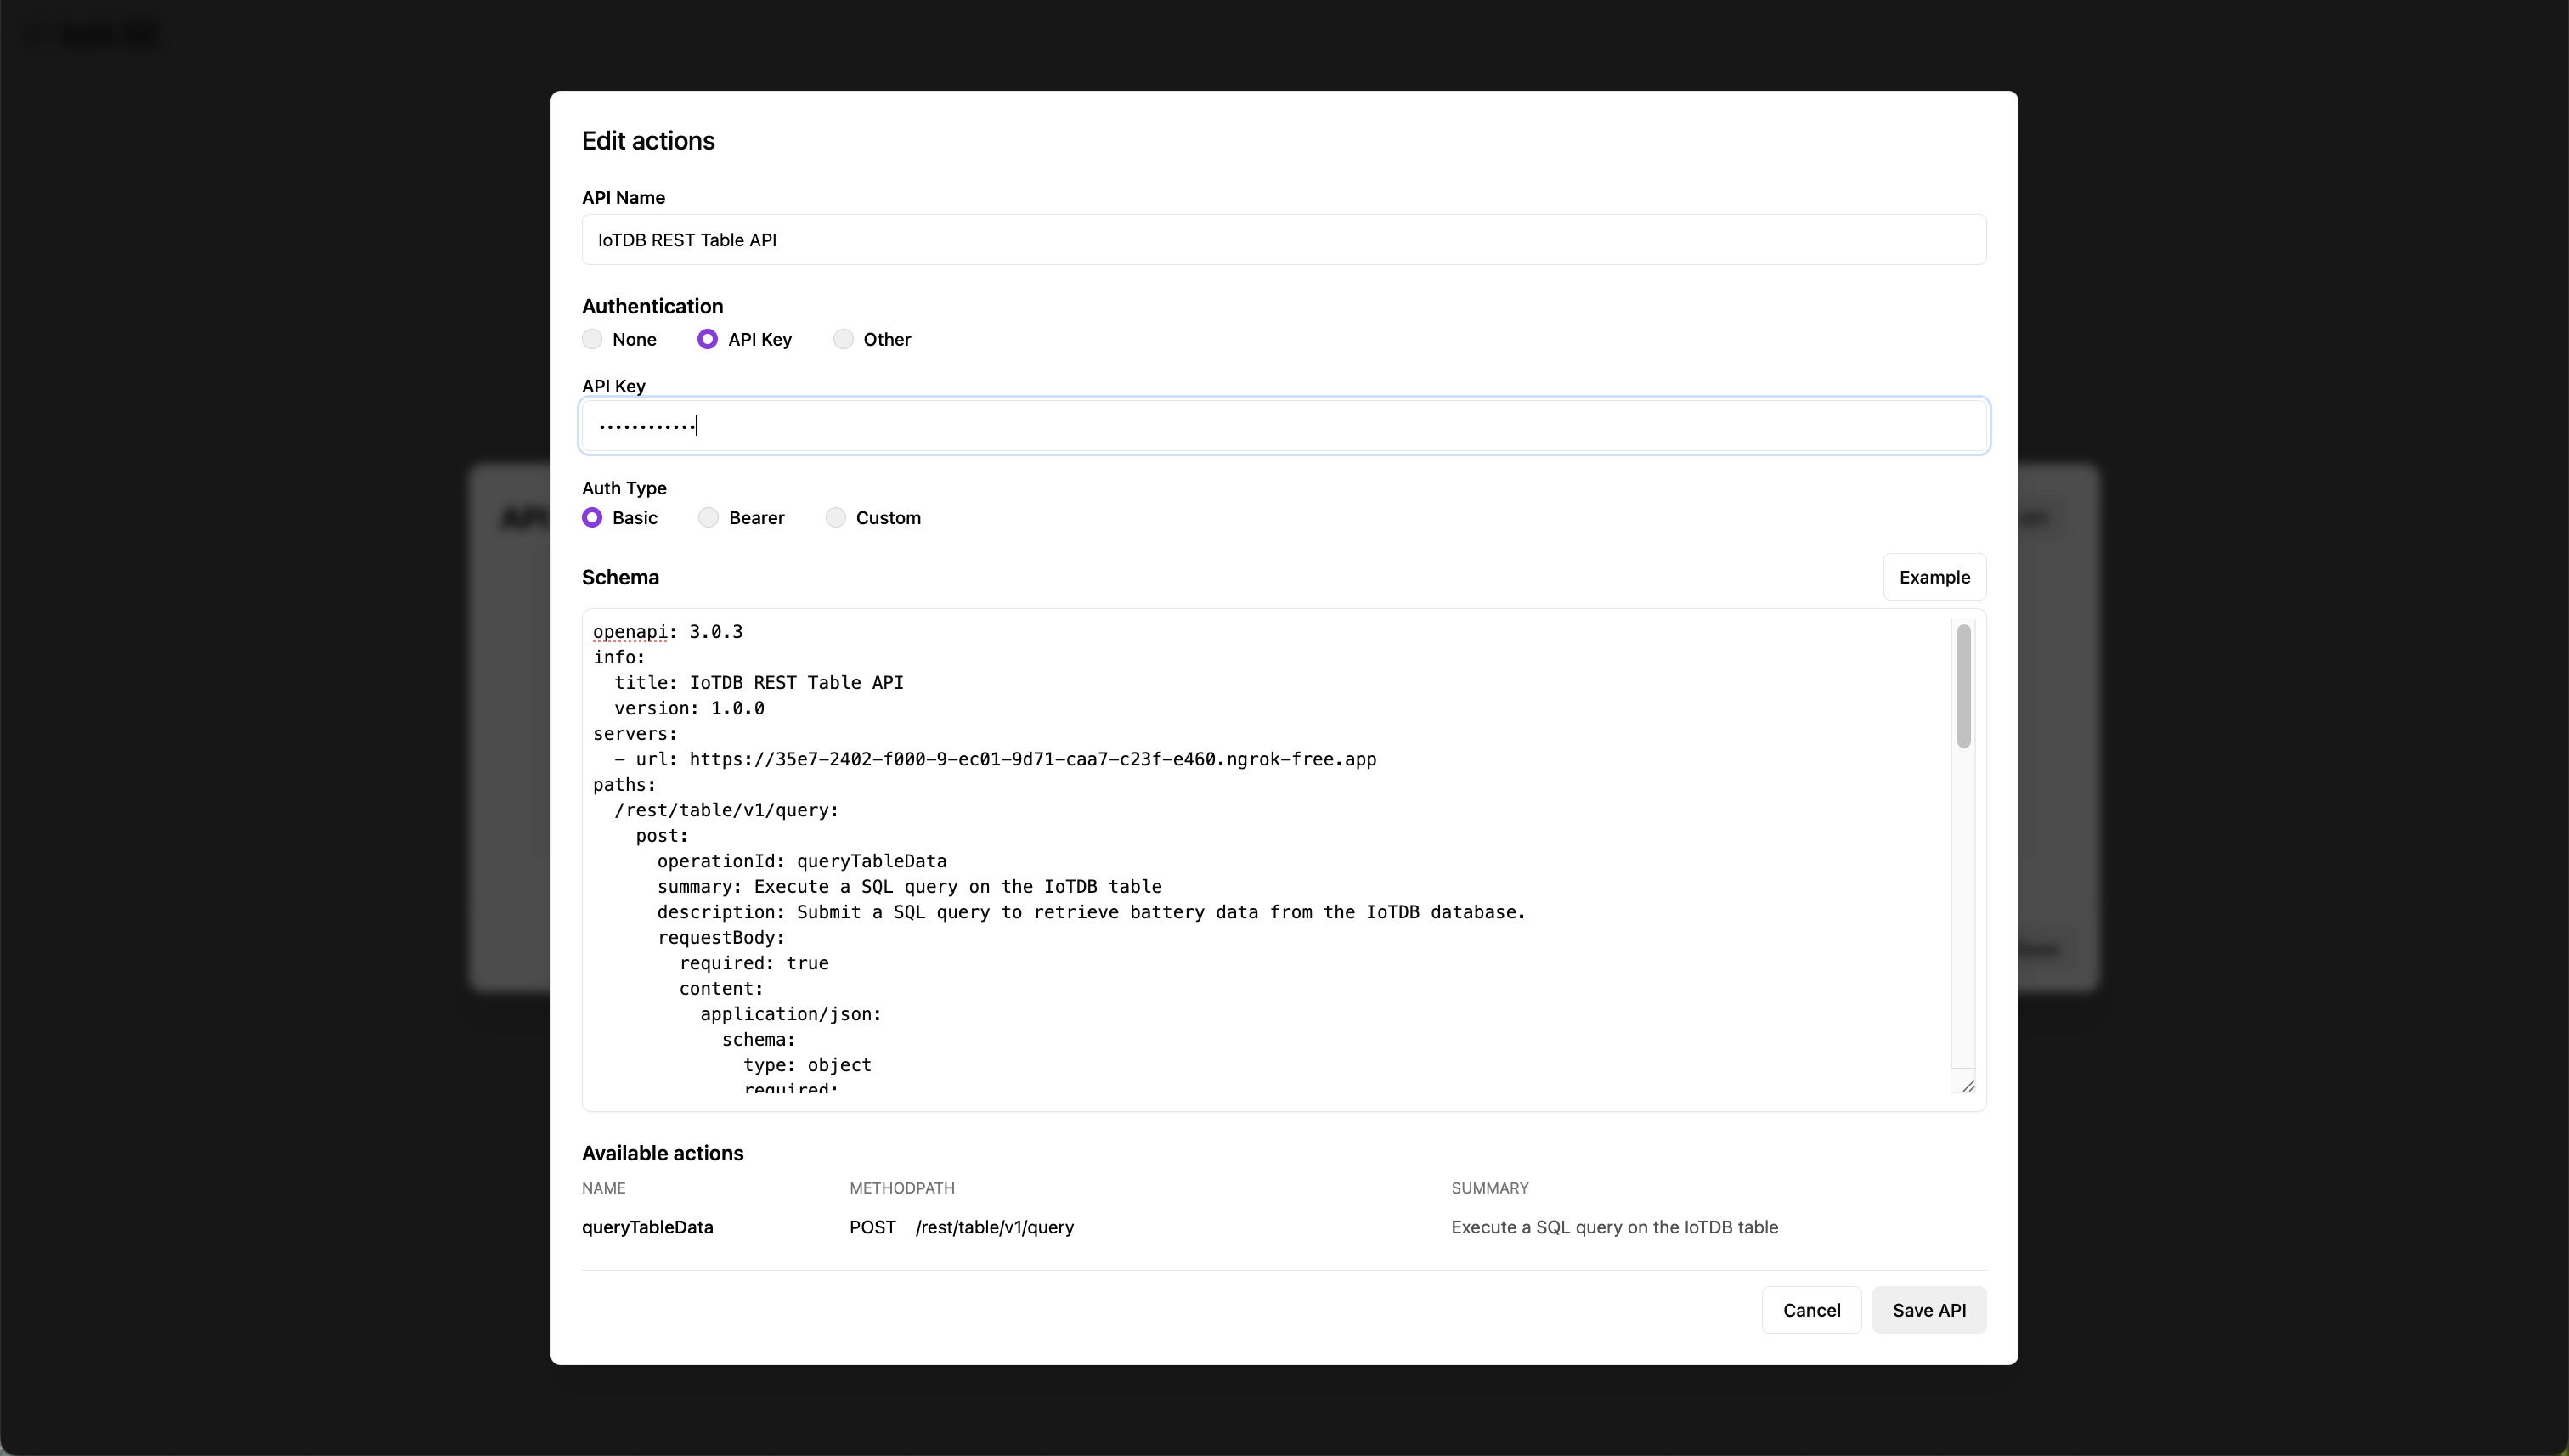
\includegraphics[width=0.8\textwidth]{figures/screenshots/iotdb-demo/openapi-editor.png}
  \caption{OpenAPI文档编辑与认证配置界面}
  \label{fig:openapi-editor}
\end{figure}

\clearpage

\begin{figure}[t]
  \centering
  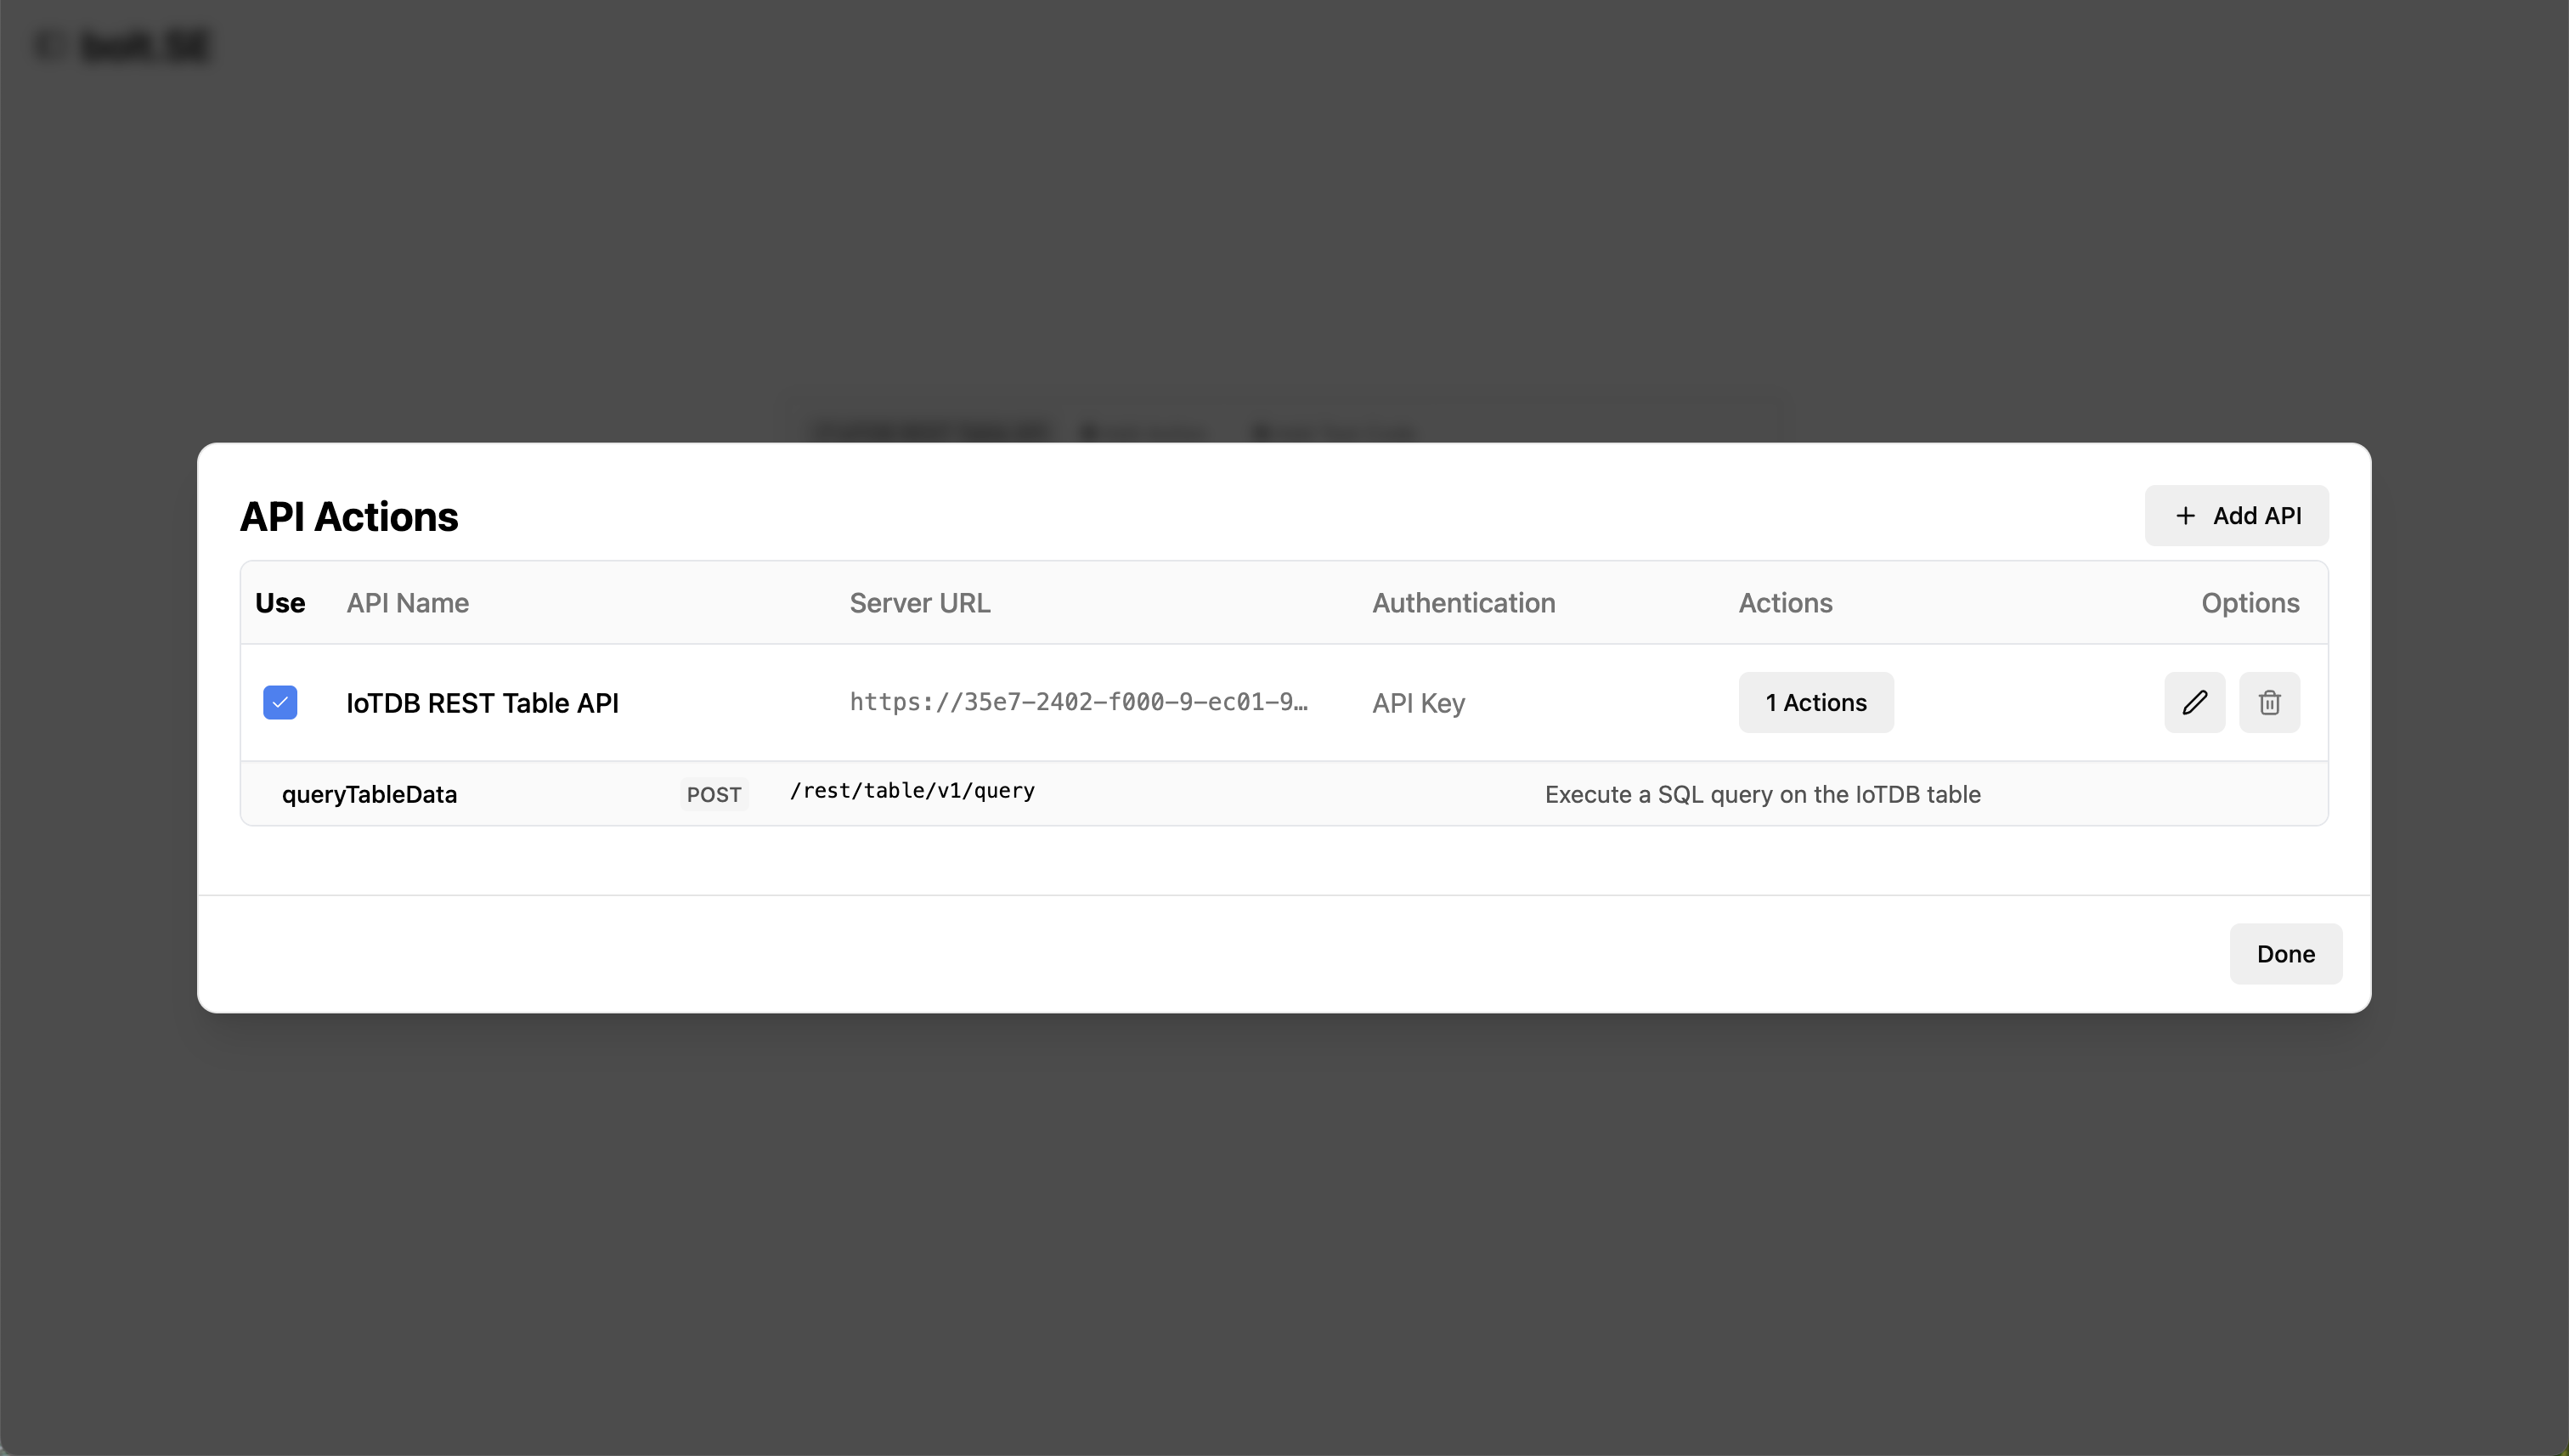
\includegraphics[width=0.9\textwidth]{figures/screenshots/iotdb-demo/api-actions.png}
  \caption{最终配置的API动作列表}
  \label{fig:api-actions}
\end{figure}

\subsection{单一自然语言提示的执行路径}

开发者向系统提交以下简洁提示:

\begin{quote}
\small
\textbf{Build a basic app that displays IoTDB data in a graph. Please use the tool to check the current database structure. Add a "Reload" button to refresh the data by calling the API.}
\end{quote}

LLM首先顺序调用三个MCP工具(图~\ref{fig:mcp-call}):
\begin{enumerate}
  \item \textit{list\_tables}:确认系统中只有\texttt{battery\_data}表
  \item \textit{describe\_table}:获取表的列名及数据类型定义
  \item \textit{read\_query}:通过\verb|SELECT * FROM battery_data LIMIT 5|抽样分析数据分布
\end{enumerate}

随后调用OpenAPI动作\textit{queryTableData}构建完整查询逻辑和前端刷新机制。

\begin{figure}[htbp]
  \centering
  \begin{subfigure}{0.48\textwidth}
    \centering
    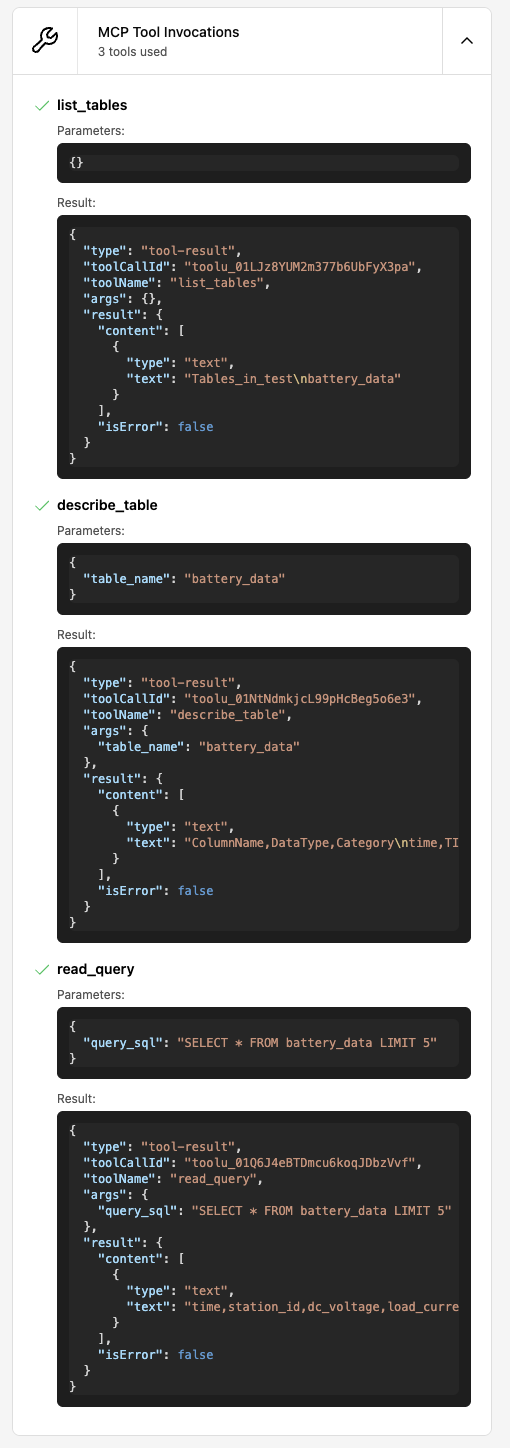
\includegraphics[width=\textwidth]{figures/screenshots/iotdb-demo/mcp-call.png}
    \caption{LLM顺序调用IoTDB相关MCP工具}
    \label{fig:mcp-call}
  \end{subfigure}
  \hfill
  \begin{subfigure}{0.48\textwidth}
    \centering
    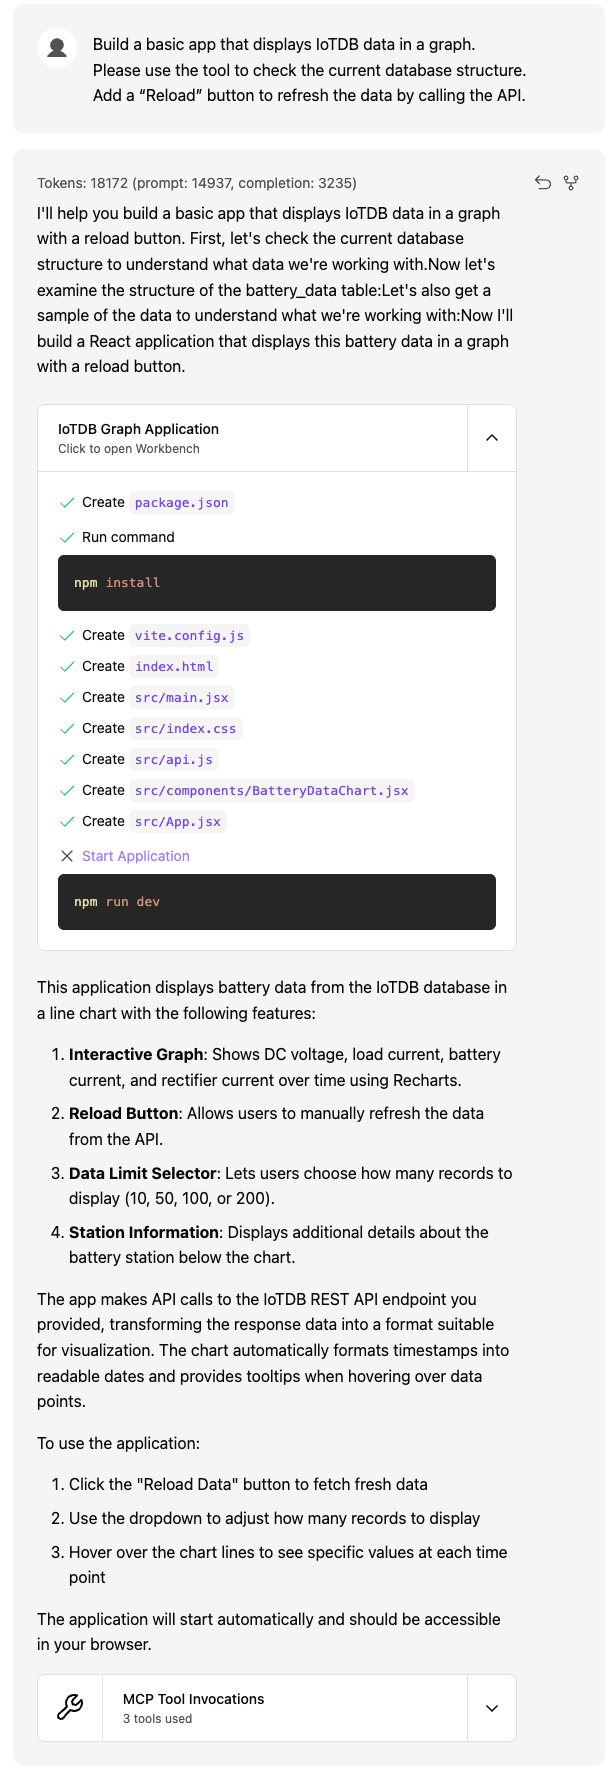
\includegraphics[width=\textwidth]{figures/screenshots/iotdb-demo/prompt-and-files.png}
    \caption{LLM回复与自动生成的文件列表}
    \label{fig:prompt-and-files}
  \end{subfigure}
  \caption{LLM工具调用与响应}
  \label{fig:mcp-combined}
\end{figure}

\subsection{自动生成的前端应用}

系统根据提示自动创建完整的Vite+React工程,包括依赖配置、文件结构和核心组件\texttt{BatteryDataChart.jsx},并在内置Workbench环境中运行。

\begin{figure}[t]
  \centering
  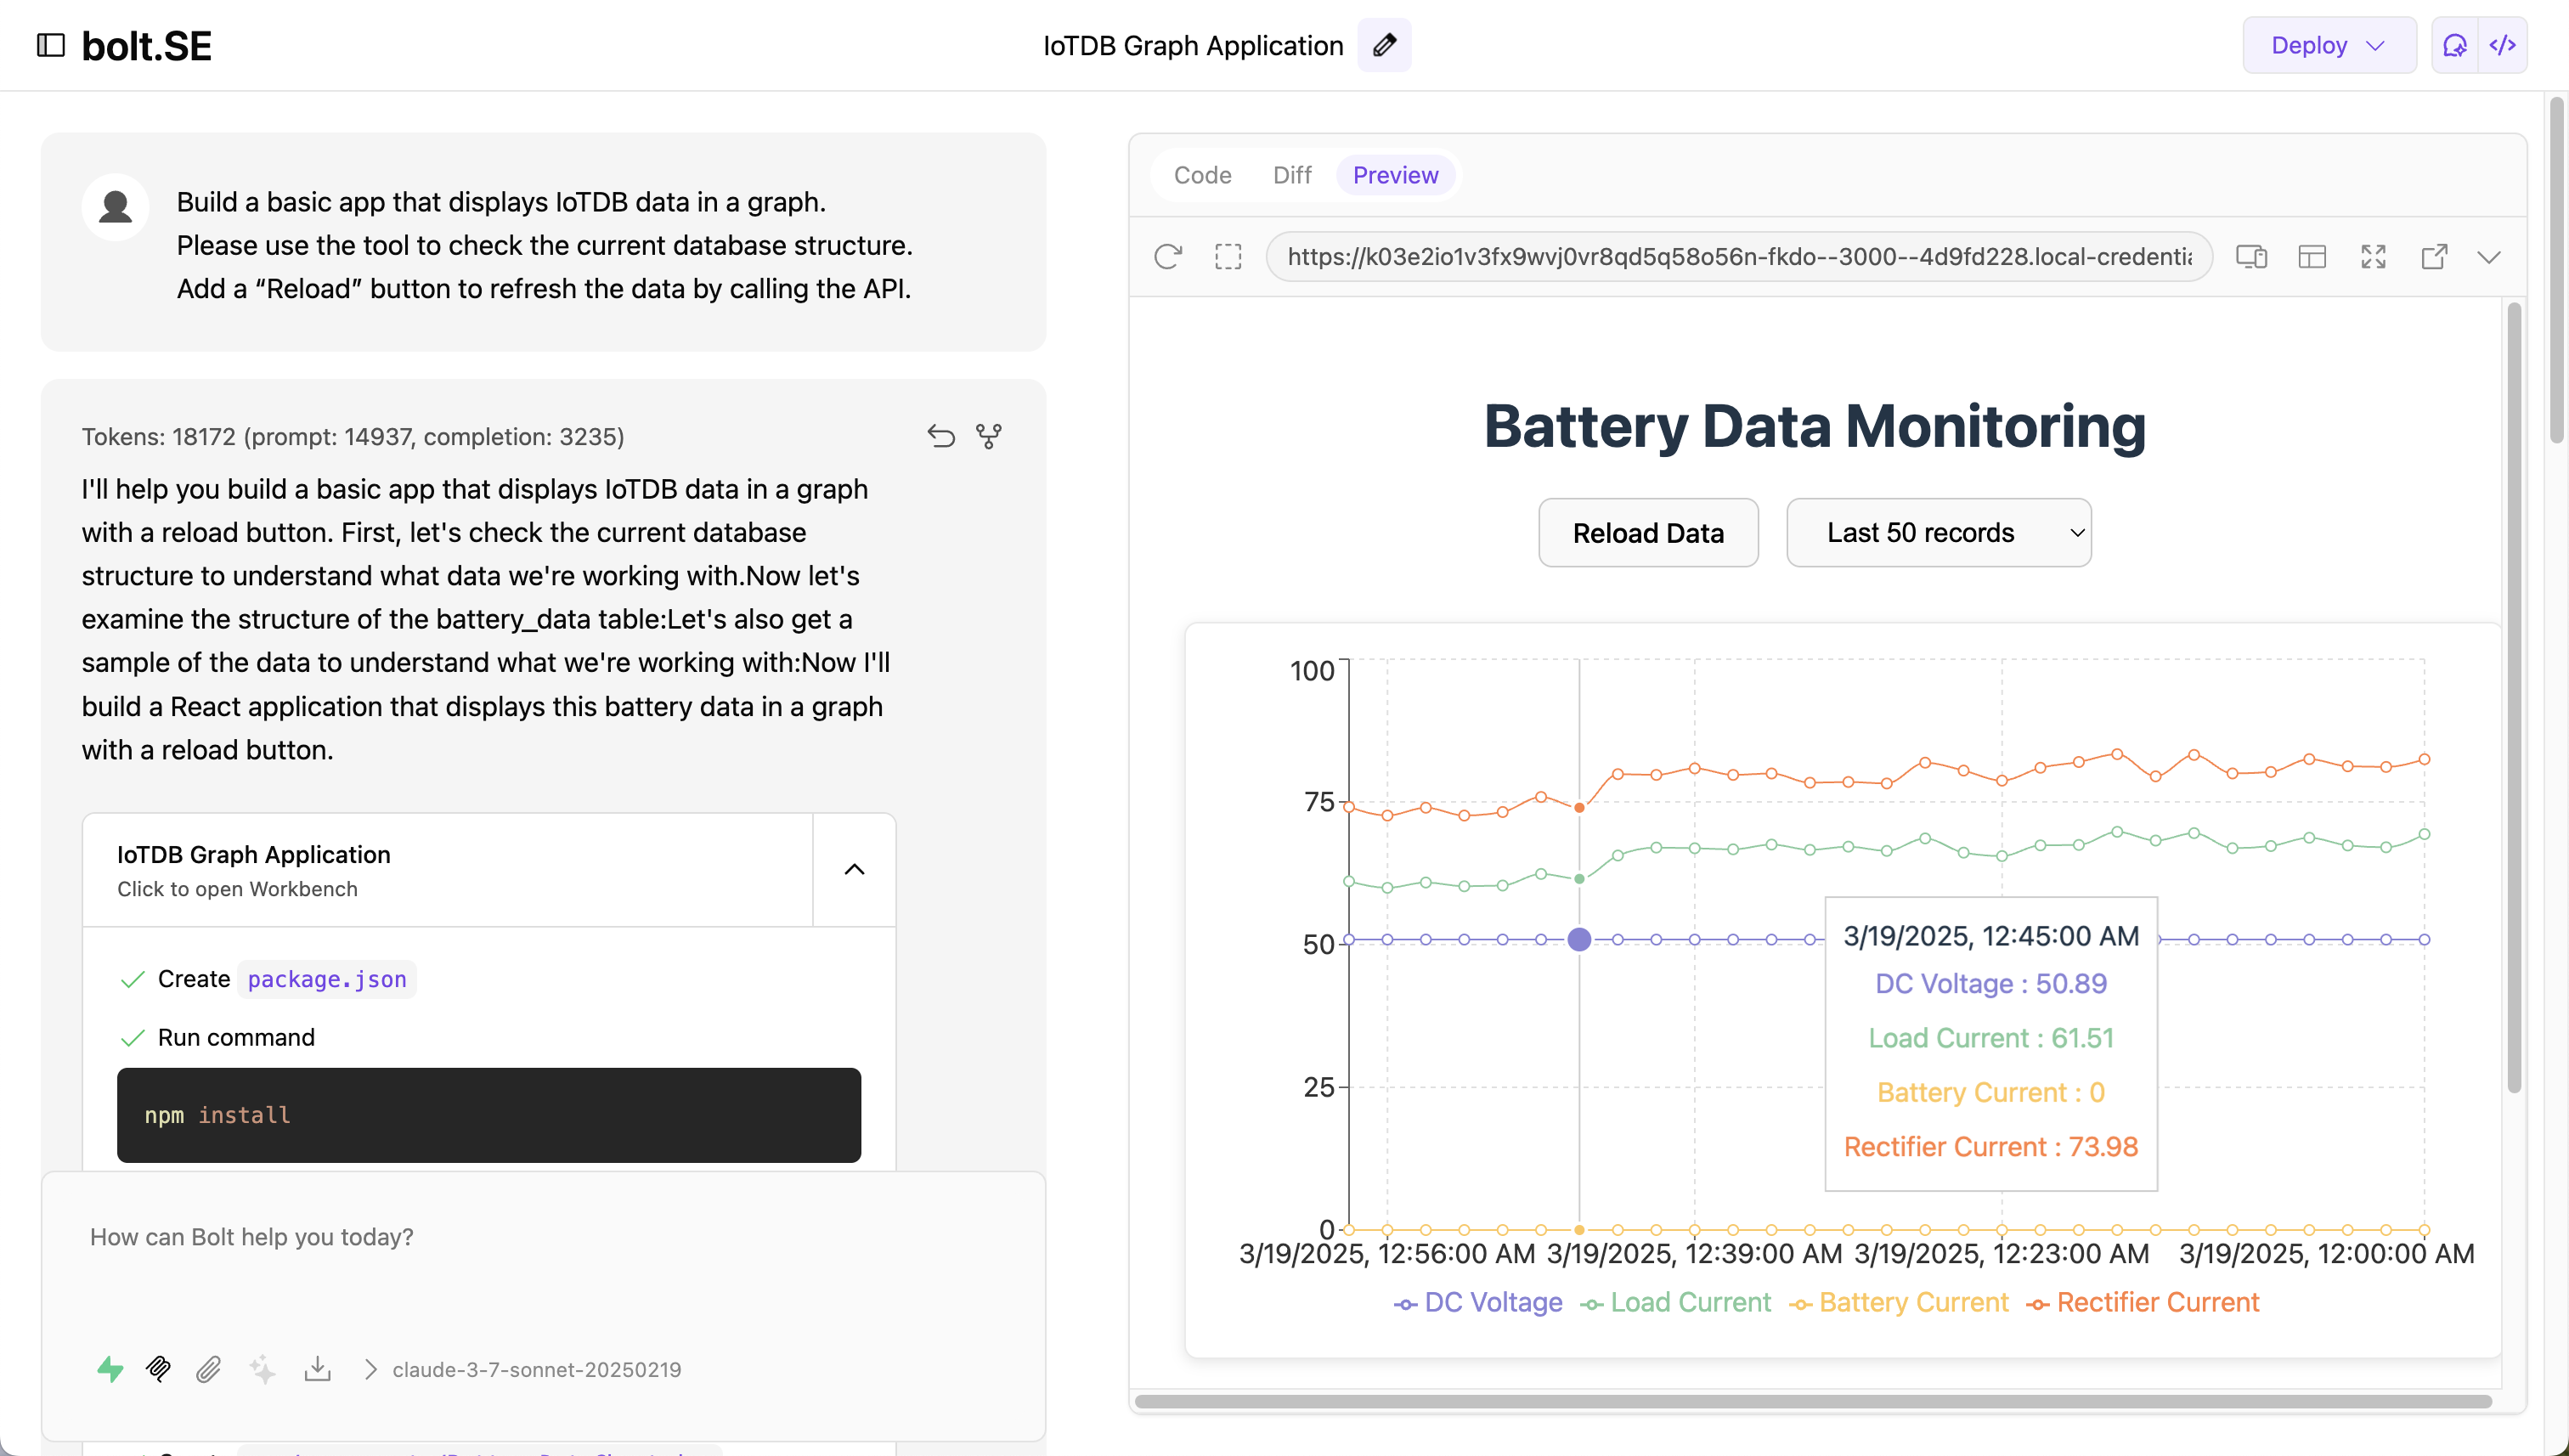
\includegraphics[width=0.75\textwidth,height=0.75\textheight,keepaspectratio]{figures/screenshots/iotdb-demo/app-preview.png}
  \caption{生成应用的Workbench预览,展示电池数据监测折线图与数据刷新功能}
  \label{fig:app-preview}
\end{figure}

图~\ref{fig:mcp-call}展示了LLM顺序调用三个MCP工具的过程,图~\ref{fig:prompt-and-files}展示了回复摘要和生成的文件列表。图~\ref{fig:app-preview}展示了最终应用界面。该应用以折线图形式展示\texttt{DC Voltage}、\texttt{Load Current}和\texttt{Rectifier Current}等数据曲线,顶部\textit{Reload Data}按钮触发\texttt{queryTableData}API调用,下拉框支持数据条数切换。